%location/filename: tex/ch1.tex
%author: Anders Østevik
%Last edited: 16.12.2015
%#######--Chapter 3--#######
%Content:
%	Interface/Communication between \acrshort{pc} and FPGA
%	

\documentclass[main.tex]{subfiles}

\begin{document}

\chapter{PC to CRU control interface} \label{chap:sercom}

In order to connect and control the \gls{cru} from a user \acrshort{pc}, some sort of serial communication between the user \acrshort{pc} and the \gls{fpga} is needed. The purpose of the serial link in this thesis is mainly to monitor and manipulate the \gls{gbt} control signals. Because of this, the speed requirements of the link is not a crucial matter. \\
Figure \ref{fig:sergui} illustrates the different blocks that make up the serial interface: The interface on the \acrshort{pc} side consists of a terminal-like interface that lets the user type in requests that enables the user to read and/or write to the \gls{gbt} control signals via the link. These requests then gets translated into byte-codes and sent out via the transmitter of the \gls{com} to the \gls{uart} on the fpga side. Here, the bytes are stored in a buffer before they get interpreted by a decoder. Depending on the user-request, the decoder can write to a \gls{gbt}-switch or read from a \gls{gbt}-probe.

\begin{figure}[H] % H(strictly put HERE > h!)
% h(here), !(force), t(top), b(bottom), p(on extra page)
\subfile{./serial_gui.tex}
\caption{Simplified diagram over the PC to CRU serial interface.}
\label{fig:sergui}
\end{figure}

\section{Readily Available Standards}
The \gls{fpga} board used in this thesis (section \ref{sec:cyclone}) has various forms of communication standards readily available. The following sections starts off with an evaluation of the different communication standards available on the \gls{fpga}, and continues with a description of the final implementation of the serial communication software and hardware.\\

When choosing the serial communication between the \gls{fpga} and the \acrshort{pc}, factors like physical compatibility, implementation, availability and complexity were taken into consideration. The \gls{fpga} board has the following communication capabilities readily available: \gls{pci}-express, Ethernet, JTAG UART (through the USB Blaster II), and an SDI-transceiver. The following short sections describe advantages and disadvantages of using one of the standards mentioned above in context with the thesis.

\subsubsection{PCI-Express}
The \gls{pci}-express connection requires the \gls{fpga} to be directly mounted on the motherboard of the \acrshort{pc}, which is in this situation impractical and not necessary for a simple communication link. This option also limits the compatibility with some \gls{fpga} boards and \acrshort{pc}s that do not have a \gls{pci}-express connection available. It does, however, enable for very fast data transmission and removes potential noise generated by using external cabling. 

\subsubsection{Ethernet}
The ethernet connection is integrated in most \gls{fpga} boards, but requires layers of protocols in order to communicate (no direct serial communication). While it is possible to send serial data over ethernet, it would require a serial-to-ethernet adapter \cite{serial2ethernet}; It would just be easier to send serial data directly from the \gls{fpga}-pins using an \gls{usbrs}-cable (see section \ref{sec:usercom}). The upside is that an ethernet connection offers long distances between the \acrshort{pc} and \gls{fpga}, either through networking or long cabling. Using ethernet for communication only requires a known IP-address between the devices for connection and transmission.

\subsubsection{SDI-Transceiver}
The \acrshort{sdi}-transceiver is meant for audio/video transmission and uses \acrshort{bnc}-connectors for this task. It therefore requires special audio/video equipment on the \acrshort{pc} side for connection and transmission, which is not necessary for a simple communication link.

\subsubsection{Altera JTAG}
Serial communication through the Altera JTAG UART IP is possible through the only \acrshort{usb}-connection on the board; the USB Blaster II, which is primary used for programming the \gls{fpga}. This requires the implementation of the Nios II soft processor. A soft processor is a microprocessor implemented into the \gls{fpga} with the help of logic synthesis only. While it is also possible to use a \gls{hps}, only a few \gls{fpga}-boards (SoC-boards) comes with one implemented. There is no support for \gls{hps} on the \gls{fpga} board used in this thesis. A Nios II-extension for the Eclipse \acrshort{ide} in combination with the C programming language is commonly used to program the soft processor. Using this approach not only limits the user to send and receive data through a dedicated Altera System Console \cite{altera_terminals14}: the Nios II also occupies a large portion of the \gls{fpga}.

\begin{figure}[H] % H(strictly put HERE > h!)
% h(here), !(force), t(top), b(bottom), p(on extra page)
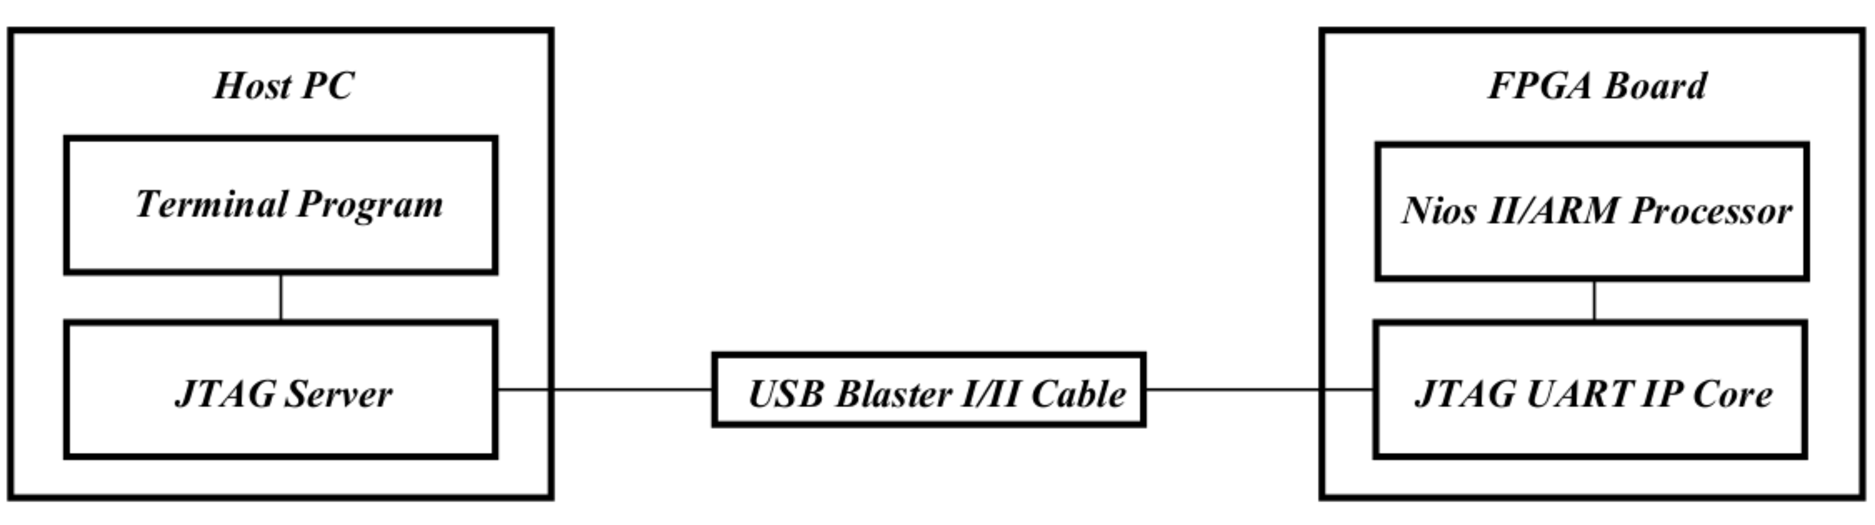
\includegraphics[width = 12 cm]{../img/altera_jtag}  \\[0.1 cm]
\caption{JTAG UART communication link between the host PC and the FPGA board \cite[Figure 1]{altera_terminals14}.}
\label{fig:altjtag}
\end{figure}

Attempts were made to implement the Nios II and write a simple send- and receive routine in C through the Altera JTAG, but was quickly abandoned due to issues with debugging using the Eclipse Nios II \acrshort{ide}. The most serious debugging issue was the fact that the compiler continued displaying errors after the errors were corrected. Even after the actual bugged function or line of code were deleted completely, the compiler would still complain on the same errors as before it was deleted. This made the dedicated Nios II compiler unreliable, and the code impossible to debug. Not only did this approach make it a whole lot more complicated, but it was also more error prone and permitted the use of user defined software for communication with the \gls{fpga}.

\section{User Defined Communication} \label{sec:usercom}

In addition to the communication standards described above, which in turn requires specific cable- and socket types for connection, it is possible to connect the transmit and receive signals directly to the \gls{fpga} pinout. The only requirement is that the given \gls{fpga} has unoccupied transmitter and receiver signal pins available for the user; either through a HSMC-port (with the help of an additional GPIO-extension board), or through a prototype area or header.\footnote{The user has to assign the available pins to the associated transmitter and receive signals in the \textit{Pin Planner} program, as part of the Quartus II suite.}\\

The \gls{fpga} board used in this thesis has no dedicated prototyping area for external signal connection. It instead comes with an GPIO-extension board that connects to one of the two on-board HSMC-ports.\footnote{By using both the HSMC-ports on the \gls{fpga}, the GPIO-\gls{pcb} could not fit properly side-by-side with the \acrshort{hsmc}-to-\acrshort{vldb} \acrshort{pcb} (see chapter \ref{chap:pcb}) because the latter \gls{pcb} is a bit to wide.} However, if removing the on-mounted LCD-display, it is possible to use the exposed header for signaling. The header (J10 in the board schematic, as shown in figure \ref{fig:lcdheader}) is connected to a transmitter- and receiver pair (both running on a voltage of $5~\volt$), several $5~\volt$ output pins and a ground pin. By using the transmitter- and receiver pair from the available header on the \gls{fpga}, it is possible to implement a type of asynchronous serial protocol. Most \gls{fpga} developement boards, including the Terasic Cyclone GX board (see section \ref{sec:cyclone}), comes with a built-in \gls{uart}-to-USB interface. This allows you to connect the board directly to the USB-port of the \acrshort{pc} as a serial connection. The \gls{fpga} board used in this thesis has no integrated \gls{uart} interface, so this has to be implemented manually.

\begin{figure}[] % H(strictly put HERE > h!)
% h(here), !(force), t(top), b(bottom), p(on extra page)
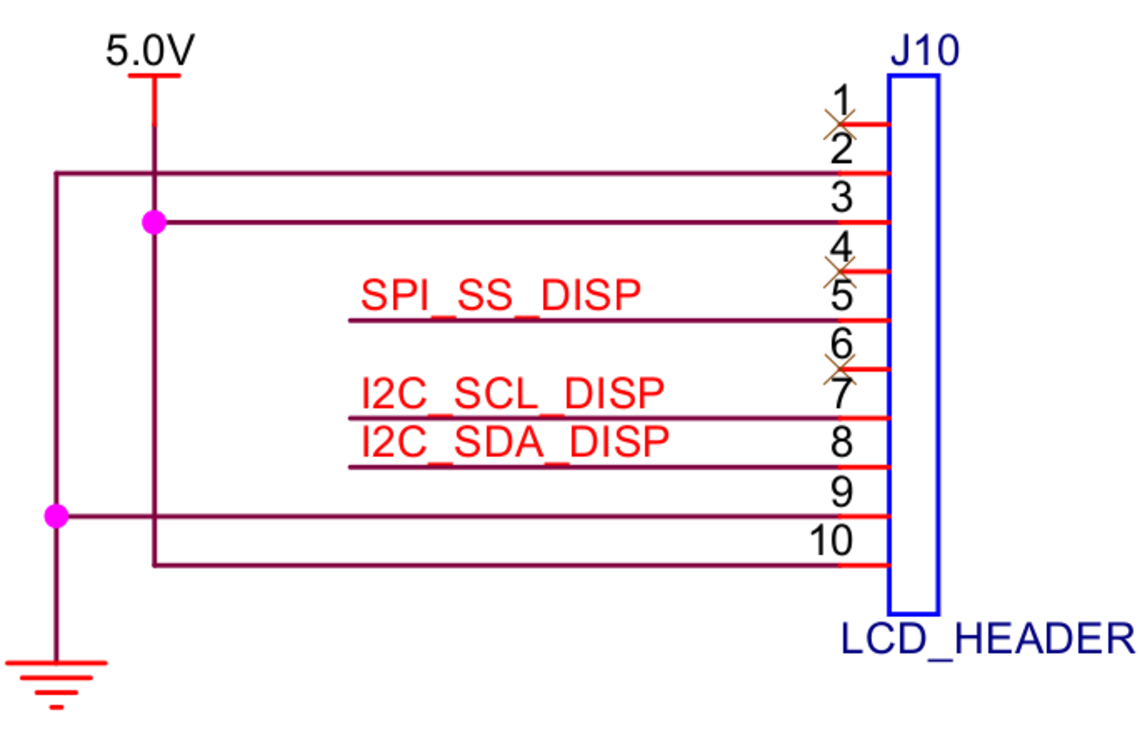
\includegraphics[width=0.5\linewidth]{../img/lcdheader.pdf}  \\[0.1 cm]
\caption{J10 header from the Cyclone V GT board schematic. The SCL and SDA signals can be used as single ended transmitter and receiver signals.}
\label{fig:lcdheader}
\end{figure}

\section{Duplex Systems}

Common to all communication systems considered is that they are all duplex systems, which simply means two connected devices that can both transmit and receive signals. While \textit{full-duplex} enables both devices to transmit and receive simultaneously (like a telephone), \textit{half-duplex} only enables one device to transmit at a time (like a walkie-talkie). Common to both the duplex systems is that they have two communication channels. 

\section{Choosing Communication Protocol}
Perhaps the most well-known and supported serial communications protocol out there is the \acrshort{rs232} standard. It supports both synchronous and asynchronous transmission, and only requires a single transmit- and receiver pair (if excluding the data control signals, which are not crucial). It is compatible over a wide range of voltage levels, and can be connected directly to the serial port of a \acrshort{pc} (if one is available) or through a \gls{usbrs}. The \acrshort{rs232}-standard was chosen mainly because it only requires two wires (one for transmitting and the other for receiving). It is supported by most \glspl{os} used today, and can be easily implemented using available C-libraries.\\

The standard will be used for asynchronous transmission of data between the \acrshort{pc} and \gls{fpga}. A simple \gls{uart} with a byte-decoder will be implemented on the \gls{fpga}-side, while a dedicated C-program with access to the \gls{com} will be implemented on the \acrshort{pc}-side. A \gls{usbrs} with a voltage converter will be used as the connection between the \gls{fpga} and the \acrshort{pc}. The following chapters describe the implementation of the serial interface, first on the \gls{fpga} side (chapter \ref{chap:hardware}) and then on the \acrshort{pc} side (chapter \ref{chap:software}).

%\chapter{Implementing a serial interface into the FPGA}


\chapter{Hardware Design on the FPGA Side} \label{chap:hardware}

\section{Specification}

The implemented hardware logic is to contain the following specifications:\\
\begin{itemize} \setlength{\itemsep}{10pt}
\item Communication with the user \acrshort{pc} using \acrshort{rs232}.
  \begin{itemize}
  \item Receive requests sent from the user \acrshort{pc}. The requests are reserved byte-codes in which the byte-decoder translates to read or write commands. 
  \item Send out data from the \gls{gbt} control-register to the user \acrshort{pc} when told. The address of the data must be specified and sent from the user \acrshort{pc}.
  \item Manage to send and receive data at a reasonable speed. 
  \end{itemize}
\item Read or write to the \gls{gbt} control-register.
\end{itemize}

\section{Hardware Components}

The below sections gives a brief description of each part of the design.\\
The \gls{uart} itself is based on the \gls{uart}-design by Pong P. Chu, found in chapter 7 from his book \textit{FPGA Prototyping By VHDL Examples} \cite{chu08}. The Baud Rate Generator is borrowed from the \textit{Uart2Bus} \acrshort{vhdl}-design by Arild Velure. The \gls{uart}-decoder was written in conjunction with the C-program on the \acrshort{pc} side, and is the one component which ties the communication together.\\

The end result forms a design that uses an \gls{uart} to receive and transmit $19200-8-N-1~$ \acrshort{rs232} data-bytes. The received bytes are stored in a \gls{fifo} until treated by the \gls{uart}-decoder. The "decoder" translates the received bytes into requests, i.e read or write requests, and manipulates or sends out data-bits from the \gls{gbt}-register according to the received requests. The \gls{uart} itself is optimized for $19200~\bit\per\second$, but has been tested to work at speeds up to $57600~\bit\per\second$.

\subsection{UART}
For communication with the user \acrshort{pc}, a simple \gls{uart} was implemented into the \gls{fpga}.\\
Simply put, an \gls{uart} is a circuit that transmits and receives parallel data through a serial line \cite{chu08}. It uses the concept of oversampling to synchronize with the incoming data. This involves using a sample-clock which is 16 times faster than the transmitted/received data.\\

The \gls{uart}-design is divided into five parts:
\begin{itemize}
\item A Receiver that receives the serial data and reassembles it into parallel data.
\item A Transmitter that sends parallel data bit by bit out the serial line.
\item A Baud Rate Generator that generates the right amount of ticks relative to the baud rate and global clock.
\item Two \gls{fifo}-registers connected to the transmitter and receiver to shift the data in or out.
\end{itemize}

\subsection{UART Oversampling and the Baud Rate Generator}

To obtain an accurate sampling of the received signal, an asynchronous system like the \gls{uart} uses what is referred to as oversampling. \\

With a typical rate of 16 times the baud rate, the receiver listens for the line to go from idle to the first start bit. When pulled low or high (depending on the system), a counter starts counting from 0 to 7. When the counter reaches 7, the received signal is roughly in the middle of the start bit. By sampling the bit in the middle of its time frame, the receiver avoids the noise and ringing that are generated whenever a serial bit changes \cite{rapid08}. When in the middle of the start bit, the counter needs to tick 16 times before it reaches the middle of the first data bit, the \gls{lsb}. The \gls{lsb} can now be sampled, and the procedure is repeated $N - 1$ times until reaching the last data bit, the \acrshort{msb}. If there is a parity bit, the same procedure is repeated one more time to retrieve it. After retrieving all the data bits, the same procedure is used one last time to sample the M stop bits at the end of the signal. After this, the line is held high until a new start bit arrives. 

%\mdfdefinestyle{mystyle}{rightmargin=90pt, linecolor=darkgray}

\begin{figure}[!htp]
\begin{center}
%\begin{minipage}[!h]{0.85\linewidth}  %Needed this to lign the figures up properly
%\begin{mdframed}%[style=mystyle]
\begin{tikztimingtable}[%
    timing/dslope=0.5,
    timing/.style={x=1ex,y=4ex},
    x=4ex,
    timing/rowdist=5ex,
    %timing/coldist=2ex,
    xscale=0.8,yscale=0.7, % scale diagrams
    timing/name/.style={font=\sffamily\scriptsize}
    ]
\\
Data      & 14h 28l 28d{$d_0$} 28d{$d_1$} 28d{$d_2$} \\%16d{$d_3$} 16d{$d_4$} 16d{$d_5$} 16d{$d_6$} 16d{$d_7$} 16d{$stop$}H \\
Sample ticks        & h 125{c}\\
\\
%\vspace{20pt}
%AD   & 2u 1D{addr} 1U{} 1D{$d_1$} D{$d_1 '$} D{$d_2$} 2D{$d_3$} U \\
%C/BE & 2u 1D{0010} 6D{BE\#} U  \\
%IRDY      & UU 4L HLH \\
%TRDY       & UU HLH 3L H \\
%DEVSEL     & 2U 6L H\\
\extracode
\begin{pgfonlayer}{background}
\begin{scope}[semithick]
\vertlines[darkgray, dotted]{1.75, 3.5}
\vertlines[darkgray,dotted]{7.0, 10.5,...,14}
  
  \draw[<->] (1.75,-10) -- (3.5,-10) node [midway,below] {\scriptsize 8 cycles};
  \draw[<->] (3.5,-10) -- (7.0,-10) node [midway,below] {\scriptsize 16 cycles};
    \draw[<->] (7.0,-10) -- (10.5,-10) node [midway,below] {\scriptsize 16 cycles};
      \draw[<->] (10.5,-10) -- (14.0,-10) node [midway,below] {\scriptsize 16 cycles};

  \draw[<-] (3.5, 1) -- (3.5,2) node [midway,above] {\scriptsize Middle};
 \draw[] (3.5, -2.6) -- (3.5,-2.6) node [midway,above] {\tiny Start bit};
  \draw[<-] (7, 1) -- (7,2) node [midway,above] {\scriptsize Sample LSB};
  \draw[<-] (10.5, 1) -- (10.5,2) node [midway,above] {\scriptsize Sample d1};
  \draw[<-] (14, 1) -- (14,2) node [midway,above] {\scriptsize Sample d2};

\end{scope}
\end{pgfonlayer}
\end{tikztimingtable}
%\end{mdframed}
\caption{\gls{uart} receive synchronisation and data sampling points with 16 times the sampling rate.}
\label{fig:uartsample}
%\end{minipage}
\end{center}

\end{figure}

To achieve a sampling rate of 16 times the baud rate, a Baud Rate Generator module is implemented into the design. The module generates a one-clock-cycle tick once every $\frac{clock}{16 \times baud\ rate}$ clock cycles. This is achieved by counting in certain steps given by the formula below:

\begin{equation}
Baud\ frequency = \frac{16 \times baud\ rate}{GCD(clock, 16 \times baud\ rate)}
\end{equation}

, where baud frequency is the count steps, and \textit{GCD} is the greatest common divisor between the global clock and the baud rate times 16 \cite{velure10}. \\
For a baud rate of $19200\ \bit\per\second$ and a clock of $50\ \mega\hertz$, the counter must count in steps of $96$ per clock cycle. 

Once the counter reaches a given baud limit, the counter resets and the tick-signal is pulled high. After one clock cycle, the tick-signal is pulled low and the counter starts to count upwards again. The baud limit is given by:

\begin{equation}
Baud\ limit= \frac{clock}{GCD(clock, 16 \times baud\ rate)} - baud\ frequency
\end{equation}

, where clock is the global clock of the system and GCD is the greatest common divisor between the global clock and the baud rate times 16 \cite{velure10}. \\
For a baud rate of $19200\ \bit\per\second$ and a clock of $50\ \mega\hertz$, the counter must count in steps of $96$ up to the baud limit of $15565$, before pulling the tick-signal high and start over again. 

\subsection{UART Receiver}
The receiver is essentially a finite state machine, divided into four states: the idle-, start-, data- and stop state. It uses the Start and Stop bits to reset the state machine in an attempt to synchronize the clock phase to the incoming signal. For this, the receiver contains three registers: the s- and  n registers for counting, and a b register for data storing. The s-register keeps track of the sample ticks and n-register the number of data bits sampled.
There are two constants defined for the receiver: the $C\_DBIT$ constant, which indicates the number of data bits; and the $C\_SB\_TICK$ constant, which indicates how many ticks that is required for the stop bit(s) (16 ticks for 1 stop bit). 

\begin{figure}[!htp]
\begin{center}
%\usetikzlibrary{arrows,automata}
\begin{tikzpicture}[>=stealth',shorten >=1pt,auto,node distance=4cm]
  \node[initial,state,accepting] (idle)      {\small{\textit{idle}}};
  \node[state,accepting]         (start) [right of=idle]  {\small{\textit{start}}};
  \node[state,accepting]         (data) [right of=start] {\small{\textit{data}}};
  \node[state,accepting]         (stop) [right of=data] {\small{\textit{stop}}};
 
  %\path[->]          (S)  edge [loop above] node {a} (idle);
  \path[->]          (idle)  edge [loop above] node {} (idle);
  \path[->]           (idle)  edge              node {\small{\textit{rx = '0'}}} (start);
  \path[->]          (start)  edge [loop above] node {\small{\textit{s = s+1}}} (start);
  \path[->] (start) edge             node {\small{\textit{s = '7'}}} (data);
  \path [->]             (data) edge [loop above] node {\small{\textit{n = n+1}}} (data);
  \path[->] (data) edge             node {\small{\textit{n = C\_DBIT-1}}} (stop);
  \path [->]             (stop) edge [loop above] node {\small{\textit{s = s+1}}} (stop)
             edge [bend left]  node[align=center] {
             \small{\textit{s = C\_SB\_TICK-1}} \\ \small{\textit{rx\_done\_tick = '1'}}
             } (idle);
\end{tikzpicture}
\caption{\gls{uart} receiver state machine.}
\label{fig:uartrx}
\end{center}
\end{figure}

\subsubsection{Idle state}
Starting with the idle state: given that there is not already a signal being received and sampled (i.e $rx\_done\_tick = '1'$), the receiver waits for the rx-signal to go low (i.e detecting a start signal). The s-register then resets and the state machine goes to the next state: the start state. 

\subsubsection{Start state}
When in the start state, the ticks generated by the baud rate generator clocks the s-registers and waits for it to count up to 7 (i.e in the middle of the start-bit). It then resets the s- and n-registers and sets the next state to the data state. 

\subsubsection{Data state}
Since the received signal so far is the middle of the start bit, the s-register must count up to 15  before reaching the middle of the data bit so that the b-register can sample the data. Each time the s-register reaches 15, the b-register shifts in the rx by 1 bit while the n-register increments by 1, keeping track of the bit width. When the n-register reaches a count equal to the $C\_DBIT$ constant minus 1, the transmission is at its end, and the state machine shift to the last state: the stop state. 

\subsubsection{Stop state}
The stop state uses the sample ticks in conjunction with the s-register to count the stop bit(s) duration by using the $C\_SB\_TICK-1$ as the upper count limit. When done, the  $rx\_done\_tick$ signal is set to 1 and the state machine shifts back to the idle state. We have now successfully received a serially  transmitted byte. %The state machine is shown in figure \ref{fig:uartrx}. 

\subsection{UART Transmitter}
The \gls{uart} transmitter has a similar design to that of the receiver; it uses the same state machine structure, but for the purpose of shifting out data. In addition to the s-, n-, and b-registers used for counting, the transmitter contains a din-register for input parallel data and a $1~\bit$ tx-register for shifting out the data. Connected to the tx-register is a tx output signal. To prevent multiple clocks, the baud rate generator is also used to clock the transmitter. For the transmitter to be properly synchronized with the receiver, it instead uses the counter registers to slow down the operation 16 times. This is because there is no oversampling involved in transmitting a signal.\\

\begin{figure}[!htp]
\begin{center}
\begin{tikzpicture}[>=stealth',shorten >=1pt,auto,node distance=4cm]
  \node[initial,state,accepting] (idle)      {\small{\textit{idle}}};
  \node[state,accepting]         (start) [right of=idle]  {\small{\textit{start}}};
  \node[state,accepting]         (data) [right of=start] {\small{\textit{data}}};
  \node[state,accepting]         (stop) [right of=data] {\small{\textit{stop}}};
 
  %\path[->]          (S)  edge [loop above] node {a} (idle);
  \path[->]          (idle)  edge [loop above] node {} (idle);
  \path[->]           (idle)  edge              node {\small{\textit{tx\_start = '1'}}} (start);
  \path[->]          (start)  edge [loop above] node {\small{\textit{s = s+1}}} (start);
  \path[->] (start) edge             node {\small{\textit{s = '15'}}} (data);
  \path [->]             (data) edge [loop above] node {\small{\textit{n = n+1}}} (data);
  \path[->] (data) edge             node {\small{\textit{n = C\_DBIT-1}}} (stop);
  \path [->]             (stop) edge [loop above] node {\small{\textit{s = s+1}}} (stop)
             edge [bend left]  node[align=center] {
             \small{\textit{s = C\_SB\_TICK-1}} \\ \small{\textit{tx\_done\_tick = '1'}}
             } (idle);
\end{tikzpicture}
\caption{\gls{uart} transmitter state machine, similar to that of the receiver.}
\label{fig:uarttx}
\end{center}
\end{figure}

\subsubsection{Idle state}
When in the idle state, the tx-register is held high for idle line and the b-register is connected to the din register for data input. The state machine remains in the idle state until the $tx\_start$ signal changes from low to high. It then shift to the start state to begin the transmission of the data stored in the b-register. 

\subsubsection{Start state}
When in the start state, the tx-register is held low for the start bit to be transmitted out. When the s-register reached the count of 15, the start bit is transmitted and the state machine shifts to the data state to further transmit the actual data bits.

\subsubsection{Data state}
When in the data state, the tx-register is set to the first bit of the b-register, while the b-register shift its data using a simple right shift operation every 16 clock ticks (s-register reaches 15). To keep track of how many data bits that have been transmitted, the n-register increments by 1 at the same rate as the b-register shifts the data (same as for the receiver). When reaching $C\_DBIT-1$, the data bits is finished transmitting out and the state machine shifts to the stop state.

\subsubsection{Stop state}
When in the stop state, the tx-register is held high indicating a stop bit is being transmitted. When the s-register reaches a count equal $C\_SBIT - 1$, the stop bits are finished transmitting. The $tx\_done\_tick$ signal is set to high and the state machine shifts back to the idle state, ready to transmit the next data byte.

\subsection{FIFO Buffers}
Both the \gls{uart} transmitter and receiver has \gls{fifo}-buffers that stores the incoming data sequentially in a "First In, First Out" manner. On the receiver side, the incoming data is stored until it gets the read-out signal ($rd\_uart$ goes high). It then places the first stored byte on the ($r\_data$)-line for one clock cycle. As long as the read-out signal remains high and there is bytes stored, the \gls{fifo} will spew out data on the ($r\_data$)-line with the rising edge of the clock. The $rx\_empty$ signal indicates whether there is one or more bytes stored in the \gls{fifo}. On the transmitter side, when data from the \gls{fpga} is written into the \gls{fifo}, it sends a signal to the transmitter to start shifting out the data stored in the buffer, oldest byte first. Having \glspl{fifo} to store data between the \gls{uart} and the rest of the \gls{fpga} logic is necessary to prevent data loss, as the \gls{fpga} logic operates at a much higher clock speeds than the \gls{uart}  can transmit and receive data. If a \gls{fifo} gets filled up, no new data will be written to it until data is read out of it, freeing one slot.

\subsection{UART Decoder}
The \gls{uart} decoder is a state machine connected to the other end of the \gls{uart} receiver- and transmitter \glspl{fifo}. It reads out the received bytes and does tasks according to the order and value of the bytes. Starting at the idle state, the decoder waits for a request byte from the fifo followed by an address byte. The request byte can for instance be a read or a write. The following small sections describes the different decoder states. 

\subsubsection{Idle state}
Being initially in the idle state, the decoder is triggered by the $rx\_empty$ signal coming from the rx-fifo, which is held low if there is at least one byte stored in the rx-fifo. If $rx\_empty$ is low, the decoder sends a read signal ($rd\_uart$), telling the rx-fifo to place the next in-line byte on the read-bus ($r\_data$), and in the same delta-time assigns the read-bus to a new register ($b\_reg(0)$) for temporary storage. The decoder then goes to a read state.

\subsubsection{Read1 state}
 In the read1 state, the first temporary stored byte is analyzed. The byte must have a value that is equal to one of three predefined constants, called requests (See $uart\_gbt\_pkg.vhdl$). This first byte is interpreted as a read- or write-request, sent from the client \acrshort{pc} through the serial connection. If the request-byte is equal to a "read" request, a "write 0" request or a "write 1" request, the decoder goes on to a wait state. If the byte is not a request-value, the state machine returns back to idle and reset the registers.

\subsubsection{Wait1 state}
  In the wait1 state, the decoder waits for the next arriving byte after the first one. The wait state does the same as the idle state, i.e waits for $rx\_empty$ to become low before reading out the next byte from the rx-fifo. To prevent the state machine from getting stuck in the wait state (if an address byte does not arrive in time), an additional count-register, triggered by the baud generator ticks, counts up to a predefined value, $C\_TIMEOUT$. $C\_TIMEOUT$ is defined to be a reasonable larger value than the pre-estimated time it takes for the next byte to arrive, i.e $16 ~ticks\per\bit \times 10 ~bits$. If $rx\_empty$ is not triggered low before the count-register has finished counting, the state machine resets to idle. If the next byte arrives before timeout, the decoder stores it and goes to the final state.

\subsubsection{Read2 state}
  In the read2 state, the value of the first byte, the request-byte, decides if the decoder should perform a read or a write operation on the gbt-register. The value of the last received byte is treated as an address to the data of the gbt-register the client wants to read or write to.  


\chapter{Software on the PC Side} \label{chap:software}

The program was written with the goal of one day replacing the Quartus-bound In-System-Source-And-Probe Editor, which is used today to access the \gls{gbt} control-signals; and instead introduce a cross-platform, open-source solution.

To access the serial port on the \acrshort{pc}, the software uses free and cross-platform C-libraries (see sections below).

The C programming language was chosen for this task mainly because of previous experience with the language, but also because of desire to learn to use the language more professionally. 

\section{Specification}

The program is to contain the following specifications:\\
\begin{itemize} \setlength{\itemsep}{10pt}
\item The ability to send and receive bytes from the \gls{uart} on the \gls{fpga}. 
\item An user interface that makes it easy to control and monitor the \gls{fpga}, i.e a command console.
\item Cross-platform. This was not a critical requirement, but was added later because of the language the program was written in and also the already cross-platform libraries used. 
\end{itemize}

\section{Software Structure and Flowchart}

The software is divided into two modules; one module for sending and receiving data, to and from the \gls{fpga}; and one module that acts as the actual software interface. Both these modules were intended to be merged together into one program, both because of time constraints were left separated. The below sections describes the inner workings of each of the two modules, and provides flowcharts to further illustrate the behaviour.

\subsection{Interface module}
Figure \ref{fig:flowgui} illustrates the behaviour of the interface module. The main loop start by checking for any changes in screen size of the main terminal window. This allows the user to freely change the window size, although full screen is preferred. If a resize has occurred, the program stores the size-parameter and uses it to further resize and properly align all the internal windows ("Command History", "Commandline" and "Signals") using \textit{wresize}, and clears the content using \textit{wclear}. The content will later be redrawn with coordinates aligned according to the new size.\\

With ncurses, by using \textit{getch} in conjunction with \textit{nodelay}, one can check for key-presses without having to pause the entire program (see \ref{sec:ncurses}). If a key is pressed, the program analyses the input: If a character is typed, it is appended to a command-string and displayed in the "Commandline" window. 

If it is a return-character ('\textbackslash n'), the program processes the command-string and compares it up against a table of legal commands. The legal commands has associated functions that executes if there is a match between the input and an entry in the table. For it to be a match, the first word of the input-string must be a legal command followed by legal arguments. To see the usage of a command, one can just type in the command without any arguments. It is also possible to type in just a letter or a partial word to print out possible commands that contain the letter or partial word typed in. Legal commands include: \textit{write}, which writes a bit value to one or more of the switch-signals; \textit{read}, which sends read requests for one or more signals to the \gls{fpga}; \textit{open}, which opens the \gls{com} if it is not already open; \textit{close}, which closes the comport if it is open; \textit{status}, which prints out information about the \gls{com} and its current status; and \textit{exit}, which closes the \gls{com} and exits the program.

If either return or a character has been typed in, the program checks the input for a special key. Special keys include: "Page Up" and "Page Down", that selects which signals to display in the "Signals" window (probes, switches or both); and "Arrow up" and "Arrow down", that browse previous typed commands and displays them in the "Commandline" window.\\

After checking for key-presses, the program redraws the windows using \textit{wrefresh} and sleeps with a small delay (to prevent screen flickering and unnecessary cpu loads). It then returns to the top of the main loop and the process starts over again. 

\begin{figure}[H] % H(strictly put HERE > h!)
\begin{center}
% h(here), !(force), t(top), b(bottom), p(on extra page)
\resizebox{1\linewidth}{!}{\subfile{./flow_gui.tex}}
\caption{Flowchart over the main loop of the interface module.}
\label{fig:flowgui}
\end{center}
\end{figure}

\subsection{Send/Receive module}

Figures \ref{fig:flowtx} and \ref{fig:flowrx} illustrates the behaviour of the main transmitter and receiver functions of the send/receive module. The basic operation goes as follows: The program sends a data-pattern from a 2d-array via the \gls{com} to the \gls{gbt}-registers on the \gls{fpga} side. It then sends a read request to read all values of the \gls{gbt}-register back to confirm that the data pattern was transmittet properly. There are five different patterns that are sent in sequence to the registers, and each time a pattern is sent it is read back to the program on the PC side and displayed. This is to confirm that the communication link is working properly. \\

There are four variables that controls the transmitter: \textit{txStatus}, \textit{txReq}, \textit{txData[2]} and \textit{txAdr}. The \textit{txStatus} variable controls the behaviour of both transmitter and receiver function. For the program to be able to send a new byte out the \gls{com}, the \textit{txStatus} variable must either be flagged as idle (0x00) or as repeat (0xFD). When flagged idle, the program is not waiting for any received address-byte and is ready to transmit a new request-byte to the \gls{com}. When set to repeat, the program has already sent a request, but has not received the desired data and address byte, and must send the same read-request again. The \textit{txReq} variable determines what request is to be sent to the \gls{fpga}. When equal to a read-request (0xDD), both \textit{txStatus} and \textit{txData[0]} is set to 0xDD. If \textit{txReq} is equal to a write-request (0xEE), however, data from the \textit{GBT data table} is copied into \textit{txData[0]} using \textit{txAdr} as index. \textit{txData[1]} is set always equal to \textit{txAdr}, which is now the desired address to the \gls{gbt}-register in which to read from or write to. Sending data to the \gls{com} involves using the \textit{RS232\_Sendbuf}-function (see \ref{sec:rs232}). \textit{txAdr} is then incremented by one or reset to 0 if it exceeds the width of the \gls{gbt} data-register. If the latter is the case, it means that the read/write operation is finished, and \textit{txReq} is set to the opposite operation. If a write operation is done, the pattern index is also incremented, so that the next write operation sends out a different pattern. The transmitter function is always called before the receiver function, with a specified delay in between the two function calls. \\

\begin{figure}[H] % H(strictly put HERE > h!)
\begin{center}
% h(here), !(force), t(top), b(bottom), p(on extra page)
\resizebox{0.8\linewidth}{!}{\subfile{./flow_tx.tex}}
\caption{Flowchart over the transmitter function.}
\label{fig:flowtx}
\end{center}
\end{figure}

For the receiver function to read out what is stored in the \gls{com} buffer, \textit{txStatus} must be set to read (0xDD). The process of reading out a byte from the \gls{com} involves using the \textit{RS232\_PollComport}-function (see \ref{sec:rs232}). The \textit{n} variable is equal to the number of bytes read from the \gls{com}. If no bytes are present, this means that the previous read-request has not been received or processed properly by the \gls{fpga} \gls{uart} state machine. \textit{txStatus} is therefore set equal to repeat (0xFD), signaling the transmitter function to send the same previous read-request to the \gls{com}. If \textit{n} is larger than 0, the data and address values are filtered out of the byte(s); the data bit being the \gls{msb} and the address the remaining bits.

\begin{figure}[H] % H(strictly put HERE > h!)
\begin{center}
% h(here), !(force), t(top), b(bottom), p(on extra page)
\resizebox{0.7\linewidth}{!}{\subfile{./flow_rx.tex}}
\caption{Flowchart over the receiver function.}
\label{fig:flowrx}
\end{center}
\end{figure}


\section{Conclusion and Discussion}

As for now, the serial interface software consists of two modules: the sending and receiving module, and the ncurses command interface. Both modules work  more or less as they should: The send/receive module writes a pattern to the \gls{gbt}-register in the \gls{fpga} and reads it back to the terminal, and the interface module allows you to perform write- and read-commands and monitor the \gls{gbt} control signals. What remains is to fully integrate the send/receive module into the interface module. The module is partly integrated in terms of merging the two programs. What is left undone is to rewrite the main transmit and receive routines from the send/receive module, which are not completed. In addition, some adaptations needs to be made to the write- and read command-entries in order for them to invoke and direct the send/receive module. Also, a final test of the software as a whole remains.

% \subsection{Notable Problems}

% To keep the \gls{gbt}-register persistent with the data-pattern, the software has to continuously write to it. Tests were conducted were the software would send a write-pattern only once, and then read it back continuously: When running the software over a period of time, certain bits would at random times switch back to their initiated values. For instance, if the data-bit of address "x0C" is initiated '0' when the \gls{fpga} is turned on; when written a '1' to it by the software, it would change back to '0' after a random period of time if it is not written to again. This seemed to occur more often for certain bits than others, but when running the software in "read-only" for longer periods of time, more and more bits would eventually switch back to their initiated values. The problem seemed to become worse at higher baud rates. However, when the program kept writing to the register after every read, the bits would remain at the desired values.\\

% When writing input-strings in the commandline of the interface module, one can only use \textit{backspace} and \textit{enter} to get rid of the string that is typed in. \textit{Backspace} removes the last character typed in, and \textit{enter} will result in the program trying to execute the typed-in string and then remove it completely from the commandline (and respond with an error if the string does not match any built in commands). Attempts were made to implement similar behaviour found in linux-terminals: using the keyboard buttons, \textit{up} and \textit{down}, to copy previous written commands into the commandline, and use the \textit{left} and \textit{right} buttons to move the cursor in between the characters of the string. While the \textit{up} and \textit{down} commands are usable, scrolling between characters with \textit{left} and \textit{right} did not work very well, and the functionality were left out. 

\end{document}